\subsection{Оптимизация системы охлаждения ГТУ}
Одной из особенностей проектируемой ГТУ является предварительное захолаживание воздуха, охлаждающего турбину высокого
давления, во внешнем воздухо-водяном теплообменном аппарате. Данная конструкция позволяет сильно уменьшить температуру
охлаждающего воздуха (с 771 К - температура нв выходе из КВД до 500 К - температура на входе в ТВД). Кроме того,
вывод охлаждающего воздуха за пределы корпуса позволяет также использовать дожимающий компрессор для увеличения
давления воздуха, что позволит осущестлять его выдув в лобовой точке соплового аппарата турбины высокого давления.

Схема установки с дожимающим компрессором представлена на рис.~\ref{img:sub_compress_scheme}.

\begin{figure}[H]
    \centering
    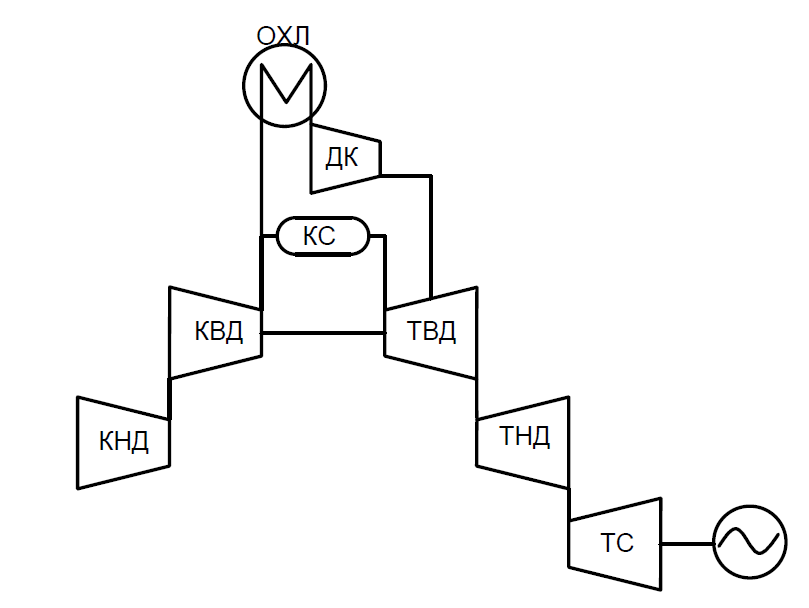
\includegraphics[scale=0.6]{sub_compress_scheme}
    \caption{Схема установки с дожимающим компрессором}
	\label{img:sub_compress_scheme}
\end{figure}

В данной работе был проведен анализ эффективности этого конструктивного решения, с точки зрения параметров установки на номинальном режиме, а также с точки зрения оптимизации системы охлаждения. 

Подробный расчет системы охлаждения соплового аппарата приведен ниже.

При оценке влияния дожимающего компрессор на цикл установки, его параметры принимались следующими: степень
повышения давления $\pi_{д.к.} = 1,2$, а его КПД $\eta_{д.к.} = 0,78$.
Расход воздуха через дожимающий компрессор определялся из условия обеспечения наибольшей температуры металла соплового аппарата 1000 К (графики распределения температуры будут показаны ниже).

Без выдува в лобовую точку относительная доля охлаждающего воздуха, отводимого из компрессора высокого давления, составляет 10\%, что в абсолютном значении составляет 5,11 кг/c. Применение дожимающего компрессора позволило уменьшить эту величину до 9,64\%, что в абсолютном значении составляет 4,92\%.

Сравнение параметров исходной установки и установки с дожимающим компрессором представлено в табл.~\ref{tab:sub_compress_comparison}.
\begin{longtable}{|c|c|c|c|}
	\caption{Сравнение параметров исходной установки и установки с дожимающим компрессорм}
	\label{tab:sub_compress_comparison}
	\hline
	\textbf{$\pi_к$} & \textbf{$\eta_e$} & \textbf{$L_e, \ МДж/кг$} & \textbf{$G_в, \ кг/с$} \\ \hline
	19 & 0,382 & 0,305 & 51,1 \\ \hline
	19 & 0,380 & 0,304 & 51,1 \\ \hline
\end{longtable}
При этом на привод дожимающего компрессора тратится $N{e \ д.к.} = 169 \ кВт$, что составляет 1\% от номинальной мощности
установки.

Как можно заметить, использование дожимающего компрессора приводит к небольшому снижению КПД установки, однако данное снижение представляется оправданным в связи с уменьшением температурной неравномерности в материале соплового аппарата турбины выского давления (показано ниже).